\documentclass{article}
\usepackage{graphicx}
\usepackage{listings}
\usepackage{xcolor}
\usepackage{geometry}

\begin{document}
\begin{titlepage}
    \centering
    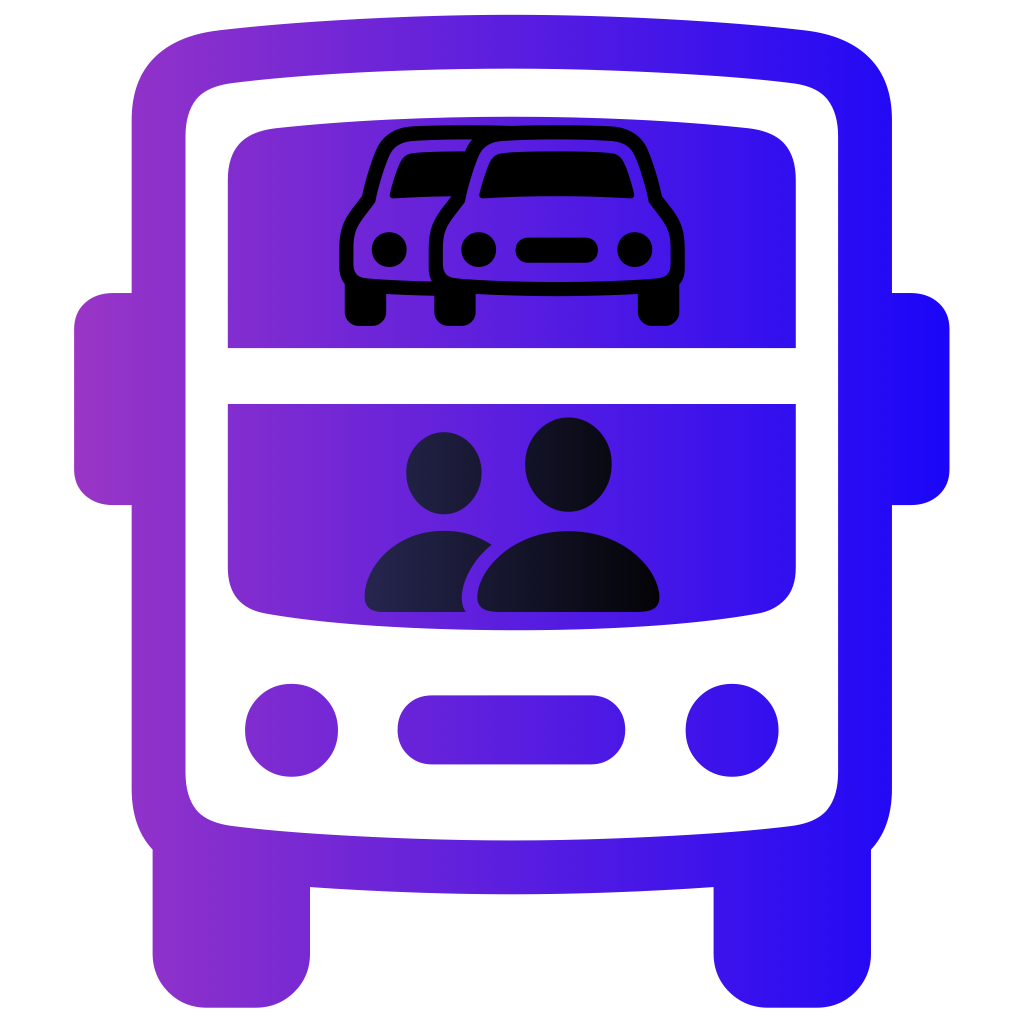
\includegraphics[width=0.5\textwidth]{logo.png}\par\vspace{1cm}
    {\scshape\LARGE UberLand City \par}
    \vspace{1cm}
    {\scshape\Large Addressing Transportation Challenges \par}
    \vspace{2cm}
    {\scshape\LARGE The Tech Support Titans\par}
    \vspace{.6cm}
    {\itshape\LARGE Rayan Mubarak,  Maadhav Deekshitha, Vinesh Ramroop, Greg Roudenko\par}
    \vfill
    {\large \today\par}

\Large\textbf{GitHub Repository:} \\
    \Large\url{https://github.com/rayannm/UberHackathon}
\end{titlepage}


\tableofcontents


\section{Abstract}


UberLand is a city with a population of over 5 million people and is a hub for businesses, tourism, and cultural events. The city faces heavy traffic congestion during peak hours. In this document, we explore this challenge and propose a solution. The solution includes creating an efficient connection between public transport and ride sharing to decrease the amount of private vehicles. In addition to this, we used A* algorithm and data sets to optimize the efficiency of routes when navigating to a destination. We also added accessibility features to cater to as many users as possible. We also created a User Interface for easy use and increased accessibility.

\section{Integration with Public Transport}
Seamless integration between ridesharing and public transit is crucial to make transportation within the city of UberLand efficient. By combining these two forms of transportation, we can limit the use of private vehicles. Private vehicles, although convenient for individual travel, have become a significant contributor to traffic congestion. In a city where roads are already strained, each private vehicle on the road exacerbates the problem, leading to longer commute times, increased greenhouse gas emissions, and diminished overall quality of life. Moreover, private vehicles are inefficient in terms of space utilization, as they often transport only a small number of people. 

\begin{figure}[h]
    \centering
    \includegraphics[width=.15\textwidth]{monek.png}
    \caption{Run of our A* algo}
    \end{figure}


\subsection {Our Solution}
We addressed this issue by employing the A* algorithm. A* calculates the shortest path from the starting node to the destination node while considering the weight or cost associated with each edge in the graph. We simulated a city by creating various nodes connected to represent road segments and designated sections of nodes and segments to represent downtown or major commercial zones. Each segment was assigned a random velocity based on data analysis to best simulate roads with typical congestion patterns, accounting for the central business district.

Furthermore, we replicated this process and adjusted the data according to the time of day. To seamlessly integrate public transport, we established a separate collection of nodes and segments to simulate metro stations and their respective routes. The A* algorithm was employed to calculate the most efficient combination of segments for traveling from the starting node to the end node, taking into account velocities, distances, and metro routes.

For routes involving private transportation to access metro stations, the Uber API can be used to provide price estimates and more accurately calculate travel times. This additional optimization further enhances efficiency and contributes to the seamless integration of ridesharing and public transit into a single platform.






\section{Traffic Congestion and Travel Times}


\subsection {Why is traffic congestion an issue?}


Traffic congestion is a pervasive and pressing challenge faced by urban centers around the world. It has significant impacts on residents, businesses, and the environment. One of the most immediate and noticeable effects is the increase in commute times experienced by residents which can affect both their personal and professional lives by causing frustration and reduced productivity. 

It can lead to substantial economic costs for both individuals and businesses. Delays in shipments and longer delivery times can disrupt supply chains and increase operational costs, which can result in higher prices for goods and services.

The environment is also greatly affected by traffic congestion. Congested roadways often result in vehicles idling for extended periods, which increases emissions of pollutants and greenhouse gases such as carbon monoxide (CO), carbon dioxide (CO2), nitrogen oxides (NOx), and particulate matter. 

\begin{figure}[h]
    \centering
    \includegraphics[width=0.4\textwidth]{Figure_1.png}
    \caption{Average vehicles on an hourly basis}

    \includegraphics[width=0.4\textwidth]{Figure_2.png}
    \caption{Traffic congestion on a juction over time}

\end{figure}
\subsection{Our solution: }

Our first step in approaching the problem was to collect data, for this we used FEDESORIANO's  \textbf{{Traffic Prediction Dataset}} we wrote python scripts, and used various libraries like MatPlotLib and the data sets to  figure out the following: 
\textbf{{a.}}  to stochastically  assign random velocities to various road segments within the city \textbf{{b.}} the peak times that we would need to factor into our A* algorithm. 

We simulated UberLand by designing various nodes that interconnect to represent individual road segments. Each road segment was assigned a velocity. Rather than relying on purely arbitrary velocities for road segments, we introduced stochastic velocity assignment, which was not entirely random but followed a probabilistic pattern through data analysis. Our approach factored in historical traffic data and typical congestion patterns. Furthermore, we designated specific sections to create clusters of nodes and interconnected segments to represent vital urban areas. These designated sections were strategically created by analyzing various the structure of major cities like New York City, and Miami. We also recognized the dynamic nature of traffic conditions throughout the day. Traffic conditions can vary significantly throughout the day, with rush hours and off-peak times having different congestion levels. So we systematically replicated the process and made various adjustments. This ensured that our solution remained responsive to changing traffic patterns, providing travelers with reliable routes at all hours. To create a holistic transportation ecosystem, we introduced a dedicated collection of nodes and segments to simulate metro stations and their associated routes. We utilized the A* algorithm to finally compute the optimal combination of road segments for navigating from the initial node to the final node. This calculation factored in key considerations, including velocities, distances, and the integration of metro routes, to ensure the utmost efficiency in travel planning. This approach provides commuters with a comprehensive network of transportation options based on their needs.



\section{Environmental Impact}
The environment is greatly affected by traffic congestion. One of the most pronounced effects of traffic congestion is the significant increase in the time vehicles spend idling. As vehicles inch along in bumper-to-bumper traffic, their engines continue to run, even when not in motion. This prolonged idling imposes a heavy toll on the environment. The combustion of fuel during idling releases a cocktail of harmful pollutants and greenhouse gases into the atmosphere. Among the pollutants released during idling, carbon monoxide (CO), carbon dioxide (CO2), nitrogen oxides (NOx). Carbon monoxide, a colorless and odorless gas, poses severe health risks, especially in high concentrations. Carbon dioxide, a major contributor to global warming and climate change, is emitted in substantial quantities when vehicles idle for extended periods. Nitrogen oxides, known for their role in the formation of ground-level ozone and smog, further deteriorate air quality. Particulate matter, consisting of tiny particles suspended in the air, is associated with respiratory ailments and cardiovascular diseases. Our apporach uses the A* algorithm to provide the most optimal combination of road segments for navigating from the initial node to the final node. This calculation factored in key considerations, including velocities, distances, and the integration of metro routes, to reduce the amount of private vehicles.



\section{Accessibility and Inclusivity}
\subsubsection{User Interface}
In order to be accessible to all we created a simple and efficient User Interface with an advanced JavaScript library called React.js with Next.js that works with the the native compiler of Node.js in order to render and fully compile a web page. The benefits to this rather than vanilla HTML is the fact that it is much faster, takes up less space and memory, faster to load. This is amazing as not everyone has powerful devices near them to run the A* algorithm. This is accessible for affordability. 


The goal of the User Interface was to cater to the demands of a wide range of age demographics, excelling in visual appeal and accessibility. This empathizes text-to-speech functionality, font modification, and intelligent color schemes to accommodate anyone. 

\subsection{Font Scalability}
By giving users the opportunity to customize the typeface, the program puts the user convenience at the touch of their fingers. They are able to change the text size to suit their personal wants. This allows them to improve the readability of the text, and as a result, the entire User Experience is enhanced, and especially for the elderly and/or those with visual impairments.
\begin{figure}[h]
    \centering
    \includegraphics[width=0.25\textwidth]{fontsize1.png}
    \includegraphics[width=0.25\textwidth]{fontsize2.png}
    \caption{Button for Text-to-Speech}
\end{figure}

\subsection{Text-to-Speech}
The addition of text-to-speech functionality demonstrates the applications focus on inclusive design. For users who might have reading difficulties, or simply prefer audio information, this feature is essential. The application ensures that all ages, especially the older age groups or those with reading problems, may easily, access and understand the information offered by translating on-screen text into audio. This is a truly revolutionary feature.
\begin{figure}[h]
    \centering
    \includegraphics[width=0.20\textwidth]{ertr.png}
    \caption{Button for Text-to-Speech}
\end{figure}



\subsection{Color Schemes}
The User Interface of the program includes meticulously selected color schemes to ensure that people with color vision problems are able to identify every color combination on the website. This is able to improve their capacity to understand the information being displayed. This values diversity, and takes into account the wide spectrum of people who might use, the program.


\section{Conclusion}
In conclusion, resolving UberLand City's transportation issues is crucial to raising quality of life for locals and promoting sustainable growth. Our suggested solution focuses on seamless integration of ridesharing and public transportation, makes use of the A* algorithm for route planning that is optimal, and incorporates accessibility features to serve a wide range of user demographics.

We want to lessen traffic congestion and the environmental impact of private vehicles on the road by encouraging the integration of ridesharing and public transportation. Utilizing the A* algorithm enables effective route planning that takes into account variables like traffic patterns and metro routes, thereby reducing travel times and increasing the effectiveness of all modes of transportation.

The solution is also user-friendly and accessible to a wide range of people, including those with visual impairments or reading difficulties, thanks to our emphasis on accessibility through a thoughtfully designed User Interface that includes font scalability, text-to-speech functionality, and inclusive color schemes.

By putting these ideas into practice, we hope to create a more reliable and open transportation system in UberLand City, which will ultimately improve the efficiency, environmental friendliness, and inclusiveness of the city for all its citizens

\section{Acknowledgements}

We would like to acknowledge and express our gratitude to the creators of the \textbf{Traffic Prediction Dataset} on Kaggle, made available by FEDESORIANO. This dataset has been instrumental in our data-driven approach to addressing transportation challenges in UberLand City.
https://www.kaggle.com/datasets/fedesoriano/traffic-prediction-dataset




\end{document}
